\chapter{Commutativity and Weakly Transactional Queues}
\label{commutativity}

In this chapter, we first describe the commutativity of queue operations in high-concurrent, non-transactional settings and compare it to the commutativity of queue operations in a fully-transactional setting. We then argue that the flat combining technique, while perhaps near-optimal for a highly-concurrent data structure, is no better for performance than a naive synchronization technique in a transactional data structure: this is because the flat combining algorithm's high performance comes from exploiting the greater operation commutativity present in a non-transactional setting. To demonstrate this point, we propose a transactional specification that allows greater operation commutativity with the expectation that the flat combining technique can achieve better performance under this specification. Our experimental results illustrate that the commutativity of operations in this new setting is essential for the effectiveness of the flat combining technique.

\section{Terminology}
We first introduce some basic terminology (as defined in \cite{schwarz} and \cite{weihl}) that will occur in our discussion.

\subsection{Histories}
\begin{defn}
    A \emph{history} is a sequence of \texttt{(transaction, operation, result)} tuples that represent an interleaving of operations of all committed transactions. Knowledge of both the history and initial conditions of a data structure leads to complete knowledge of the (high-level) end state of the structure and operation return values.

\begin{eg}
    \begin{lstlisting}
   
    // Q.size() == 0 
    (T2, Q.push(a), ())
    (T1, Q.pop(), true)
    (T2, Q.push(a), ())
    (T1, Q.pop(), true)
    // Final State: Q.size() == 0 
    \end{lstlisting}
\end{eg}

\end{defn}

\begin{defn}
    A history $H'$ is \emph{consistent} with $H$ if $H'$ contains the same tuples as $H$: the same transactions were executed with the same return values for all operations within the transactions.
\end{defn}

\begin{defn}
    A history $H$ is \emph{serial} if all tuples are ordered as if all transactions were executed in a serial order.
\end{defn}
\begin{defn}
    A history $H$ is \emph{serializable} if there exists a serial history $H'$ s.t. $H'$ is consistent with $H$.

\end{defn}

\begin{eg}
$H$ is a serializable history given $H'$. $H''$ represents a serial but inconsistent history with $H$.
\begin{lstlisting}
            H                       H'                      H'' 
    (T2, Q.push(a), ())     (T2, Q.push(a), ())     (T1, Q.pop(), false)
    (T1, Q.pop(), true)     (T2, Q.push(a), ())     (T1, Q.pop(), false)
    (T2, Q.push(a), ())     (T1, Q.pop(), true)     (T2, Q.push(a), ())
    (T1, Q.pop(), true)     (T1, Q.pop(), true)     (T2, Q.push(a), ()) 
\end{lstlisting}
\end{eg}

\begin{defn}
    A history $H$ is \emph{strictly serializable} and therefore \emph{valid} if it is both serializable and all operations are linearizable. Informally, this means that the serial order of transactions corresponds to the real time at which the transactions commit.
\end{defn}
\lyt{examples?}

\subsection{Dependencies}

Note that all operations can be classified as sets of reads and/or writes (as we do in Table~\ref{table:qrw}). We therefore define dependencies abstractly as reads and writes of particular objects in our definitions.

\begin{defn}
    Transaction $T2$ is \emph{dependent} on transaction $T1$ if one of the following relations holds:
    \begin{itemize}
        \item R-R: $T1$ reads an object later read by $T2$
        \item R-W: $T1$ reads an object later written by $T2$
        \item W-R: $T1$ writes an object later read by $T2$
        \item W-W: $T1$ writes an object later written by $T2$
    \end{itemize}
\end{defn}

\begin{defn}
    An operation $P$ of transaction $T1$ is \emph{commutative} with operation $Q$ of transaction $T2$ when ordering $P$ before $Q$ results in a \emph{R-R} dependency or no dependency at all.
\end{defn}

\subsection{Results}

These results are well-known in the literature about transactional data structure scalability: we repeat them here for reference.
\begin{theorem}
    A history $H$ is serializable if there are no cycles in \emph{R-W}, \emph{W-R}, or \emph{W-W} dependencies between any two transactions (see \cite{schwarz} for proof).
\end{theorem}

\begin{corollary}
    When operations commute, they can be freely ordered in the history without affecting serializability.
\end{corollary}
\begin{corollary}
    The number of valid histories of a transactional data structure is dependent on the commutativity of its operations.
\end{corollary}
\begin{corollary}
    Commutativity of data structure operations determines scalability: the greater number of valid histories, the lower the contention between transactions, and the greater the scalability of the transactional data structure. 
\end{corollary}

\lyt{examples?}

\section{Commutativity of Concurrent and Transactional Queues}

For generality, we reduce each queue operation to a read or write of a particular semantic object: the head, the tail, or the empty? predicate of the queue. This allows for our reasoning to be applied to operations that differ from our current specification of pop or push. For example, we can imagine an alternative pop operation that returns \texttt{void} regardless of whether the queue was empty, which would perform no visible reads. We summarize what reads and writes our specifications for pop and push perform in Table \ref{table:qrw}.
\begin{table}[h!]
\centering
\begin{tabular}{c||c|c}
    Operation & Read & Write\\
    \hline
    pop & empty? & head, empty?\\
    push & & tail, empty?\\
\end{tabular}
    \caption{Read and writes of queue operations}
    \label{table:qrw}
\end{table}

\subsection{Concurrent Non-Transactional Queues}


The guarantees of concurrent, non-transactional queues are \emph{nearly} equivalent to that of singleton transactions. A history of singleton transactions is automatically serializable, since the history corresponding to the ordering of operation execution is a serial ordering of transactions. The atomicity of transactions is guaranteed by the correctness properties of the concurrent data structure. However, single operations are not always linearizable: depending on the implementation of the data structure, the effects of a operation $P$ that has ``committed'' (i.e., has returned), may not be visible to an operation that is performed after $P$ returns.

The flat combining technique provides serializable, atomic, \emph{and} linearizable singleton transactions\cite{flatcombining}. Therefore, we can reason about the commutativity and therefore scalability of a concurrent, non-transactional flat combining queue using notions of transactional dependencies.

We start by defining the dependency relations between single operations (Table~\ref{table:queuesimpledeps}). A concurrent, non-transactional queue cannot have any cyclical dependencies, since such dependencies necessarily require that there exists a transaction with more than one operation. Therefore, synchronization is only necessary to ensure correctness when two threads attempt to write (W-W) or simultaneously write/read (W-R or R-W) the same object: the performance bottleneck is only caused by concurrent access synchronization. As we have shown, the flat combining approach works particularly well in a high concurrency setting to minimize the overhead of this synchronization cost.

\begin{table}[h!]
    \centering
\begin{tabular}{c||c|c|c|c}
    Object & Pop-Pop & Pop-Push & Push-Pop & Push-Push\\
    \hline
    head & W-W & & & \\
    tail & & & & W-W\\
    empty & W$^e$-R & R-W$^e$ & W$^e$-R, W$^e$-W$^e$ & \\
\end{tabular}
    \caption*{X-Y represents an operation X performed by one thread and an operation Y performed by another thread.\\$^e$ indicates that the operation modifies the empty status of the queue.\\R-R relations are not shown.}
    \caption{Dependencies of pairs of queue operations}
    \label{table:queuesimpledeps}
\end{table}

\subsection{Transactional Queues}

\begin{table}
    \centering
    \begin{tabular}{|l|l|}
        \hline
\begin{lstlisting}
1)  // Q.size() > 1 
    (T1, Q.pop(), true) // Q empty 
    (T2, Q.pop(), true) // W-W
    (T1, Q.pop(), *)    // W-W
\end{lstlisting}
        &
\begin{lstlisting}
4)  // Q.size() >= 0 
    (T1, Q.push(a), ()) 
    (T2, Q.push(a), ()) // W-W
    (T1, Q.push(a), ()) // W-W
\end{lstlisting}
\\
\hline
\begin{lstlisting}
2)  // Q.size() == 1  
    (T1, Q.pop(), true) // Q empty  
    (T2, Q.push(a), ()) // R-W
    (T1, Q.pop(), true) // W-R
    \end{lstlisting}
        &
\begin{lstlisting}
5)  // Q.size() == 0 
    (T1, Q.push(a), ())       
    (T2, Q.pop(), true)  // W-R, Q empty
    (T1, Q.pop(), false) // W-W
\end{lstlisting}
\\
    \hline
    \begin{lstlisting}
3)  // Q.size() == 1  
    (T1, Q.pop(), true)  // Q empty  
    (T2, Q.pop(), false) // W-W     
    (T1, Q.push(a), ())  // R-W     
    \end{lstlisting} &\\
        \hline
\end{tabular}
    \caption*{Interleavings that create no dependencies are left out.}
    \caption{Operation interleavings generating dependency cycles.}
    \label{tab:interleavings}
\end{table}

With a fully-transactional queue, cyclical dependencies can occur, thus reducing the number of valid histories. All possible interleavings of two transactions that generate cyclical dependencies are shown in Table~\ref{tab:interleavings}. Note that most of the interleavings that result in cyclical dependencies, and therefore invalid histories, occur only when the queue becomes empty; only when two transactions both perform pushes or both perform pops do we see cyclical dependencies in a nonempty queue. 

A transactional queue prevents these interleavings from occurring through delaying push operation execution and using a pessimistic or optimistic approach upon encountering an empty queue.

To prevent interleavings 4 and 5, all pushes are delayed until commit time. These interleavings can only occur if $T1$'s first push is visible to $T2$ prior to $T1$ committing. If we delay pushes until commit time, $T2$ will not detect the presence of a pushed item in the queue.

Because pop operations immediately return values that depend on the state of the queue (empty or nonempty), interleavings 1, 2, and 3 cannot be prevented by delaying pop operations until commit time. Instead, we can take one of two approaches:
\begin{enumerate}
    \item Optimistic: Abort $T1$ during commit time if $T2$ has committed an operation that would cause an invalid interleaving.
    \item Pessimistic: Prevent $T2$ from committing any operation until after $T1$ commits or aborts the transaction containing a pop.
\end{enumerate}

ge see the optimistic method implemented in the T-Queue1, where the \texttt{tailversion} and \texttt{headversion} are used to determine at commit time if the empty status of the queue has been modified by another, already committed transaction. The pessimistic approach is implemented in our T-Queue2, which locks the queue after a pop is performed and only releases the lock if the transaction commits or aborts, therefore preventing any other transaction from committing any operation after the pop.

In order to support transactions, the flat combining approach must do either approach (1) or (2). Here we argue that the flat combining approach cannot do either without introducing overhead that reduces its performance to below that of the T-Queue1 or T-Queue2.

If we take approach (1), a pop cannot be performed at execution time because no locks on the queue are acquired: other transactions may commit pops of an invalid head if this transaction later aborts. Thus, in order to determine if a pop should return true or if it should return false, a transactional pop flat combining request requires much more complexity than a nontransaction one: the thread must determine how many elements the queue holds, how many elements the current transaction is intending to pop, and if any other thread intends to pop (in which case the transaction aborts). The transactional push flat combining request is also significantly more complex, as it requires installing all the pushes of the transaction. Additional flat combining calls are necessary to allow a thread to perform checks of the queue's empty status (the \texttt{<EMPTY?>} flat combining call) to determine whether the transaction can commit or must abort, and to actually execute the pops at commit time. Thus, approach (1) requires adding both more flat combining calls and more complexity to the existing flat combining calls.

If we take approach (2), the flat combining approach can either perform a pop at execution time or delay the pop until commit time. If the pop is performed at execution time, then the thread must acquire a global lock on the queue after a pop and hold the lock until commit: this prevents another thread from observing an inconsistent state of the queue. If a pop should execute and remove the head of the queue prior to commit and the transaction aborts, the popped elements must be re-attached to the head of the queue. However, the cleanup procedure during an abort does not lock the queue, meaning that any other thread can commit a transaction that pops off the incorrect head of the queue. To remedy this issue, a global lock must be acquired by any transaction that performs a pop to allow for the case in which the transaction aborts. Additional flat combining calls are necessary to acquire or release the global lock. 

We can also imagine a mix of approaches (1) and (2) where if a transaction $T1$ executes a pop, we disallow any pops from other transactions (using the equivalent of a global lock) but allow other transactions containing only pushes to commit prior to $T1$ completing. This approach prevents interleavings 1 and 3, but requires performing a check of the queue's empty status, as in approach (1), if the queue is seen empty during a pop. This is because another transaction may have committed a push between the time of $T1$'s pop and $T1$'s completion. This mixed approach outperforms both approach (2) and approach (1), and is the approach described as the flat combining algorithm in Chapter~\ref{queue}. 

As noted previously, all possible approaches to prevent interleavings 1, 2, and 3 rely on additional flat combining calls and increased complexity of previously existing flat combining calls. In addition, acquisition of a global ``lock'' on the queue for approach (2) prevents the combiner thread from applying \emph{all} of the requests it sees: instead, requests will either return ``abort'' to the calling thread or not be applied, leading to additional time spent spinning or repeating requests. We see through our experiments that these changes to the flat combining algorithm reduce its performance such that it performs worse than a naive synchronization algorithm; furthermore, we claim that these changes to be necessary in order to provide transactional guarantees. The original flat combining algorithm exploits the property that any correct history of operations in data structures supporting only singleton transactions (i.e., a normal non-transactional data structure) is valid. The combiner thread is allowed to immediately apply all thread's operation requests in arbitrary order. However, this property that makes flat combining so performant disappears as soon as the algorithm has to deal with invalid histories. In the next section, we demonstrate how ignoring invalid histories leads to a version of flat combining that can outperform our T-Queue1 and T-Queue2 algorithms.

\section{The Weakly Transactional Queue} 

The Weakly Transactional Queue (WT-FCQueue) demonstrates how the flat combining technique's performance is dependent upon the number of invalid histories. This queue implements a weaker transactional specification, which provides all invariants of a concurrent queue, but provides the following guarantees instead of the transactional ones listed earlier (Chapter~\ref{queue}):
\begin{itemize}
    \item Instead of the normal pops, the queue executes \emph{LazyPops} with the following specification:
        \begin{itemize}
            \item Any two pops within the transaction do not need to pop consecutive values off the queue.
            \item A pop's return value \emph{cannot} be accessed during the transaction. The pops are applied and their return values determined only at commit time (hence the name LazyPop). 
        \end{itemize}
    \item A pop cannot remove an uninstalled value (i.e., a value pushed earlier in the same transaction).
    \item The \emph{atomic} property thus becomes: a transaction with multiple pops and multiple pushes guarantees that the operations will either all occur or that none will occur.
\end{itemize}

Given this specification, interleavings 1, 2, and 3 in Table~\ref{tab:interleavings} are allowable if the return value of the pop is not used within same transaction. This is because two pops in a transaction do not need to pop consecutive values off the queue. Interleaving 4 is prevented by installing all pushes in the same transaction together at commit time, and interleaving 5 is allowed because $T1$'s pop cannot see its earlier pushed value.

The queue under this specification retains all the fairness properties of a concurrent queue (no value remains in the queue forever, since values are still removed in the order in which they are added). Like Schwarz\cite{schwarz}, we see uses for this transactional queue as a buffer between producer and consumer activities, in which exact ordering of values in the buffer are unimportant.
Our specification differs from that of Schwarz\cite{schwarz}, however, by preventing a pop from seeing a push within the same transaction, and by preventing access to the return value of a pop until after the transaction commits. This allows us to utilize the flat combining approach to its full potential: we do not need to generate additional flat combining calls during transaction execution because the queue does not need to be accessed until commit time.

\subsection{Algorithm}

For comparison, we implement two weakly transactional queues. This allows us to determine if changes in performance are due to the changes in the transactional specification, or are instead caused by differences in synchronization algorithms.

\subsubsection{WT-Queue}
The WT-Queue uses the naive synchronization strategy from the T-Queue1 and T-Queue2. The headversion (for pops) or tailversion (for pushes) is locked prior to actually performing the push or pop at commit time. A call to pop or push at execution time does not require any access to the queue state, but merely returns a LazyPop when pop is called or adds an item to the \texttt{write\_list} when push is called.

\subsubsection{WT-FCQueue}
The WT-FCQueue uses the flat combining synchornization algorithm. We modify the nontransactional, flat combining technique as follows:
\begin{itemize}
    \item \emph{Pops}: 
    Executing a pop returns a LazyPop value. It does not generate a flat combining request or access the queue itself. At commit time, all LazyPops are instantiated with values: for each LazyPop, the thread makes a \texttt{<POP>} flat combining request. This request is completed using the vanilla, concurrent \texttt{<POP>} flat combining implementation, which simply pops an item off the queue.

    \item \emph{Pushes}: 
    Executing a push merely adds the value onto a \texttt{write\_list\_item} and does not access the queue. Pushes from the same transaction are installed together, using the \texttt{<PUSH, list>} flat combining implementation from the transactional flat combining queue that takes the entire list and pushes each value onto the queue.
\end{itemize}

\subsection{Evaluation and Results}

\begin{figure}[t]
    \centering
	\begin{minipage}{0.45\textwidth}
	    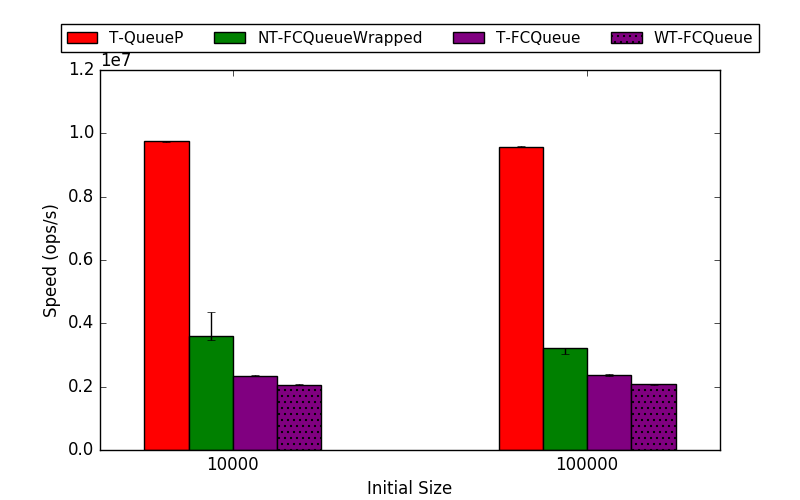
\includegraphics[width=\textwidth]{fcqueues/lpQ:PushPop.png}
        \caption*{Push-Pop Test}
	\end{minipage}
	\begin{minipage}{0.45\textwidth}
	    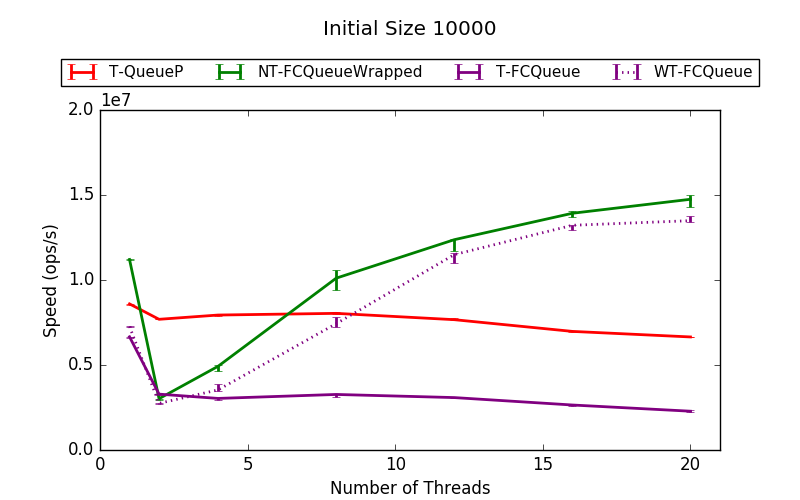
\includegraphics[width=\textwidth]{fcqueues/lpQ:RandSingleOps10000.png}
        \caption*{Multi-Thread Singletons Test}
	\end{minipage}
    \caption{WT-Queue Performance}
    \label{fig:wtqs}
\end{figure}


We evaluate the weakly transactional flat-combining queue on the same benchmarks described in Section~\ref{q_microbenchmarks} to compare against the fully transactional flat-combining queue (T-FCQueue), the T-Queue2, and the WrappedNT-FCQueue. Selected results are shown in Figure~\ref{fig:wtqs}; full results are in Appendix~\ref{app:queues}. 

While the weakly-transaction, flat combining queue (WT-FCQueue) does not perform as well as its nontransactional counterpart, NT-FCQueue, the performance of the WT-FCQueue exceeds that of the T-Queue1, the T-Queue2, and the T-FCQueue, which all provide full-transactional guarantees. We see gains in performance over the T-Queue2 up to 1.5$\times$ as the number of threads accessing the queue increases to 20; the WT-FCQueue begins to outperform the STO queue as the number of threads increases past 7. The WT-FCQueue outperforms the T-FCQueue starting at 4 threads and achieves performance up to about 5$\times$ by 20 threads.
 
The WT-FCQueue does not experience any aborts. This is due to the flat combining algorithm, which does not require that any locks be held in the weakly transactional setting in order to ensure correctness. A transaction can only abort if the result of a pop is accessed during the transaction's execution.
Because of the lack of aborts, the WT-FCQueue outperforms the T-FCQueue; this demonstrates the effectiveness of the flat combining technique in the weakly transactional setting. 

We compare the WT-FCQueue against the WT-Queue to evaluate whether performance gains comes choice of queue algorithm or instead comes from the fewer requirements of the weak transactional specification. The WT-Queue performs worse than all queues measured because of its high abort rate at commit time (100\% of aborts occur at commit time). This is caused by contention on the headversion and tailversion locks. While the actual pop function called during a transaction's execution is much simpler than in the T-Queue1 or T-Queue2 algorithms because it does not access the queue to check if the queue is empty, the installation procedure becomes more complicated because it requires instantiating all LazyPops, which more than doubles the number of cache misses from the T-Queue2.. The WT-FCQueue incurs approximately 2$\times$ more cache misses than the NT-FCQueue, but is not crippled from LazyPop-caused cache misses because the flat combining algorithm optimizes for efficient cache usage. Unlike the WT-FCQueue, the WT-Queue holds a global lock during installation at commit time, causing other transactions attempting to commit to abort. Thus, we see that the flat combining algorithm, and not the choice of transactional specification, causes the observed increased performance of the queue.

The improved performance of the flat combining algorithm on a weakly-transactional queue from that of a strongly-transactional queue demonstrates that the number of invalid execution histories directly affects the effectiveness of the flat combining algorithm. Thus, the performance of a non-transactional flat combining algorithms unlikely to be achievable in a transactional setting.

